\colorlet{jbl}{blue!65!black}
\colorlet{jgr}{green!40!black}
\colorlet{jre}{red!70!black}

\begin{block}{Cutoff effects at $\order{a^2}$}
  The higher-statistics LW ensembles let us dissect the Symanzik expansion term by
  term, comparing $\chi$ from Zeuthen versus Wilson flow and from the clover versus
  the improved charge.

  Ratios of definitions measured on the \emph{same} configurations cancel
  $\langle {\chi}_\text{cont} \rangle$ together with the action term $\langle{\chi S_{2,c}}\rangle$.
  Zeuthen flow further sets $\langle{\chi S_{2,\text{fl}}}\rangle = 0$, and the improved
  charge $\langle{\chi_2^\text{impr}}\rangle = 0$, leaving a single term in each ratio:
  %
  \begin{align*}
    {\chi^\text{Zeuthen}_\text{clover}}/{\chi^\text{Zeuthen}_\text{impr}}
      &= 1 + a^2\,{\color{jbl} \expval{\chi_2^\text{clover}}} + \order{a^4} \,, \\[0.4em]
    {\chi^\text{Wilson}_\text{impr}}/{\chi^\text{Zeuthen}_\text{impr}}
      &= 1 + a^2\,{\color{jre} \expval{\chi S_{2,\text{fl}}^{W}}} + \order{a^4} \,.
  \end{align*}
  %
  The two contributions are thus accessible separately from our data.
  \skipline
  %
  \begin{figure}
    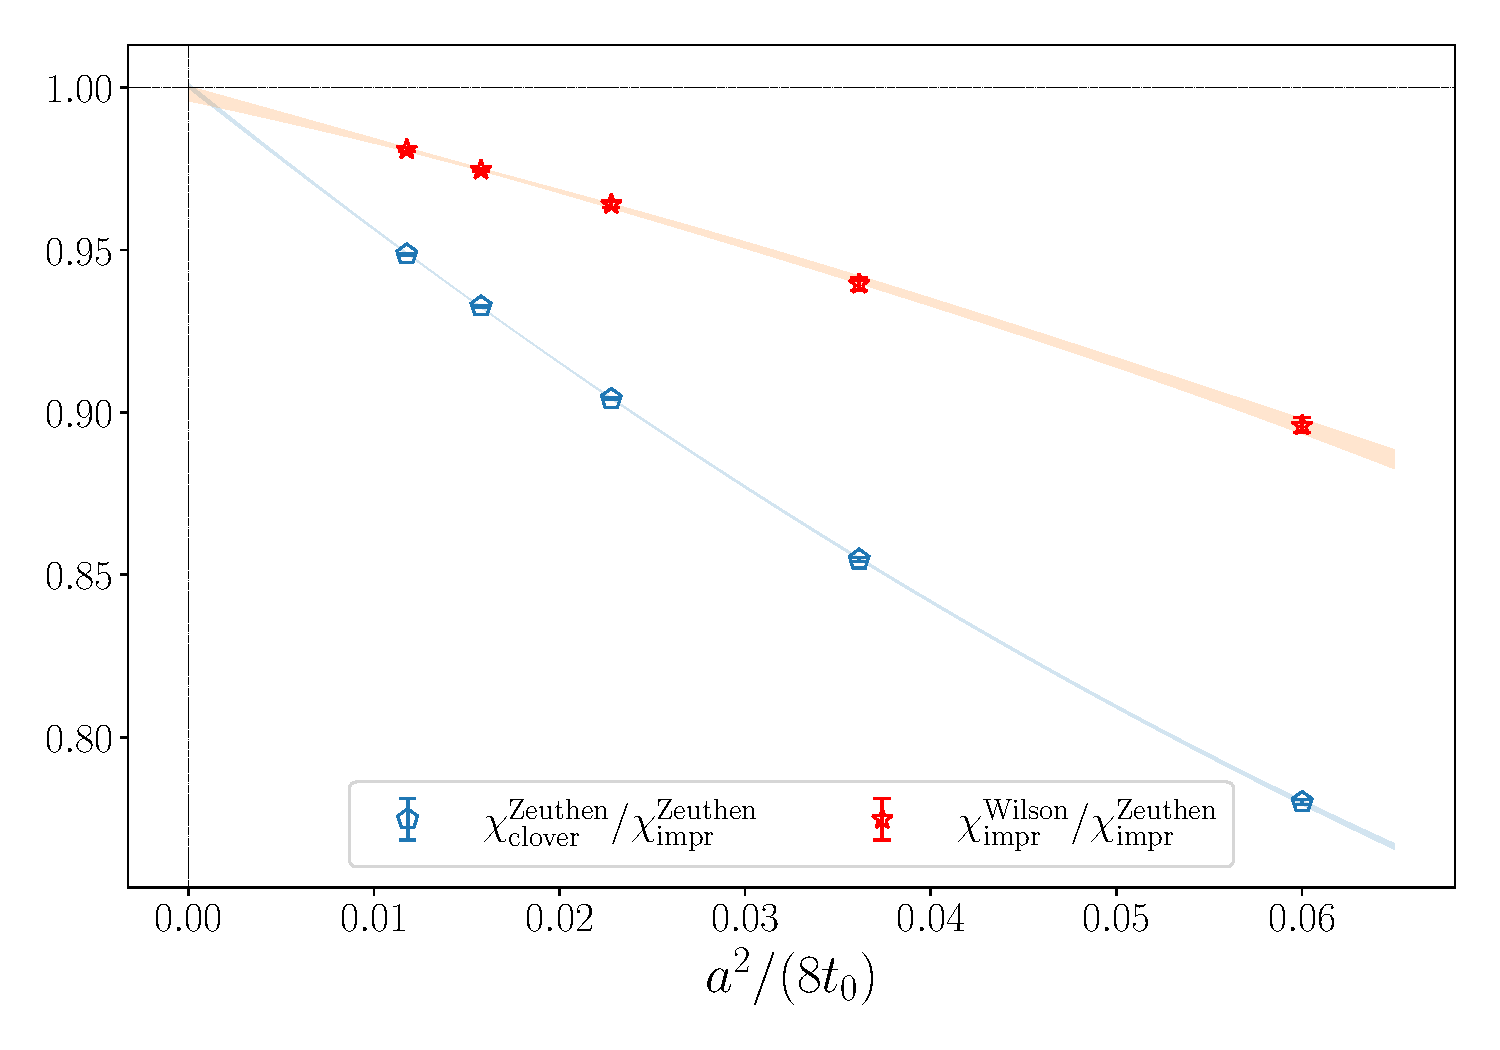
\includegraphics[scale=1.]{PLOTS/ratios_cutoff_cl.pdf}
  \end{figure}
  %
  The blue and red points isolate cutoff effects from the charge discretisation and the flow, respectively
   A quadratic dependence on $a^2$ describes the full range up to $a^2/t_0 = 0.48$,
  while a linear fit already suffices when restricted to the finest lattices. The $a^3$ contribution is therefore a small 
  but  genuine correction rather than an over-fitting artefact.

  Both ratios approach unity as $a^2 \to 0$ by construction. They quantify only \emph{classical} cutoff effects, which are cancelled exactly by combining Zeuthen flow  with the improved charge. \emph{Quantum} cutoff effects instead originate from the action used to generate the gauge configurations. The continuum-limit analysis in the left panel is designed to probe these effects, but with the present statistics and the unimproved clover charge they remain hidden within the statistical uncertainty. We plan to resolve them using Wilson-action ensembles covering the same lattice-spacing range with comparable statistics.
\end{block}